\documentclass[12pt,letterpaper,noanswers]{exam}
\usepackage[usenames,dvipsnames,svgnames,table]{xcolor}
\usepackage[margin=0.9in]{geometry}
\renewcommand{\familydefault}{\sfdefault}
\usepackage{multicol}
\pagestyle{head}
\header{AM 108 Class 25}{}{Logistic map}
\runningheadrule
\headrule
\usepackage{graphicx} % more modern
\usepackage{amsmath} 
\usepackage{amssymb} 
\usepackage{hyperref}
\usepackage{tcolorbox}

\begin{document}
 \pdfpageheight 11in 
  \pdfpagewidth 8.5in

\noindent 




\begin{itemize}
\itemsep0em
\item Project work continues next week (you'll receive feedback on your proposals, select a project, and start working on it).
\item There is a 2d system analysis due Friday Nov 13th (to be done independently - you will have access to us in office hours, but we will meet with you individually in a breakout room).
\item There is a discussion board post summary due today.
\item There will not be a pre-class assignment for Monday (there will be one for Wednesday).
\item I owe you a Quiz 02 Follow Up assignment.  Once I post it, the assignment deadline will be flexible.
\end{itemize}

\hrule
\vspace{0.2cm}



\noindent\textbf{Project Teams}

Team 1: 


\noindent \textbf{Teams 5 and 6}: Post screenshots of your work to the course Google Drive today.  Include words, labels, and other short notes that might make those solutions useful to you or your classmates.  Find the link in Canvas (or here: \url{https://drive.google.com/drive/u/0/folders/1GcpwvKHD4tMecpFQ4lNxN_r5Ylj7YHbd})


\vspace{0.2cm}

\hrule
\vspace{0.2cm}


\noindent\textbf{Big picture}

The logistic map is an important example.  We will study it (and other maps) to learn about one route to chaos and about the structure of an attractor.
\vspace{0.2cm}
\hrule
\vspace{0.2cm}

\noindent \textbf{Extra vocabulary / extra facts:}
\begin{tcolorbox}
A fixed point, $x^*$, of a map $x_{n+1} = f(x_n)$ is \textbf{stable} when $-1<f'(x)<1$.  

A fixed point of a map is called \textbf{superstable} when its multiplier, $f'(x^*)$ is zero.  

Using the Taylor series to understand the evolution of the displacement from $x^*$, with $x_n = x^* + \eta_n$, $\eta_{n+1} \approx f'(x^*)\eta_n + f''(x^*)\eta_n^2/2$.  At a superstable fixed point, this becomes $\eta_{n+1} \approx f''(x^*)\eta_n^2/2$, and convergence to the fixed point is very rapid.
\end{tcolorbox}

\begin{tcolorbox}

Assume we have a parameter, $r$, with $x^*$ and $f'(x^*)$ varying with the parameter value.  $f'(x^*) = 1$ and $f'(x^*)=-1$ indicate \textbf{bifurcations} of the map.

When $f'(x^*) = 1$, the function $f(x)$ is tangent to the line $y = x$.  This value of the multiplier is associated with a \textbf{saddle-node bifurcation}, also called a \textbf{tangent bifurcation} or a \textbf{fold bifurcation} in the context of maps.  For $f$ a smooth function, on one side of the bifurcation, looking locally, there will be no fixed points and on the other side, a pair of fixed points where one is stable and the other unstable.  In systems with a non-differentiable point, like the Lorenz map or the tent map, both fixed points might be unstable after a fold bifurcation.
\end{tcolorbox}

\begin{tcolorbox}

When $f'(x^*) = -1$, the function $f(x)$ is crossing the line $y=x$ at a right angle.  This value of the multiplier is associated with a type of bifurcation called a \textbf{period-doubling bifurcation} or a \textbf{flip bifurcation}.  In a period-doubling bifurcation, a period-2 orbit is born.  It can be either stable (existing when $f'(x^*)<-1$) in a \textbf{supercritical} bifurcation or unstable (existing when $f'(x^*)>-1$) with a \textbf{subcritical} bifurcation.

We will mainly work with \textbf{supercritical period-doubling} bifurcations and will refer to them as \textbf{period-doubling} bifurcations or as \textbf{flip} bifurcations.
\end{tcolorbox}

Again let $f(x) = r - x^2$.  The birth of two fixed points in a tangent bifurcation is visible in the sequence of plots below:

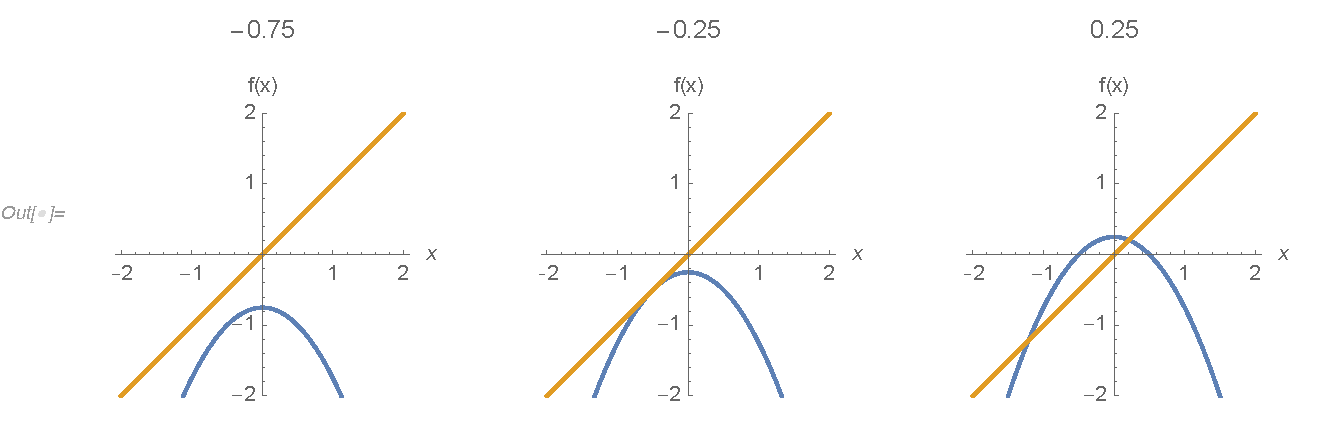
\includegraphics[width=\textwidth]{img/191105-C26p1.pdf}

The birth of a stable period-2 cycle in a flip bifurcation (at $r = 3/4$) is visible in the pair of plots below.  On one side of the bifurcation ($r = 0.73$), the orbit is "spiraling" in towards the fixed point (the side of the fixed point that it is on is going back and forth).  On the other side ($r=0.76$), a small stable period-2 orbit exists.

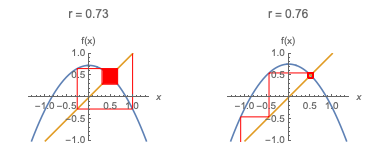
\includegraphics{img/191105-C26p3.png}


\vspace{0.2cm}
\hrule
\vspace{0.2cm}

\noindent\textbf{Skill Check C26 practice}
\begin{questions}
\item Retake of skill check C23: find the jacobian for a 3d system.

\item For the map shown below, how many period-3 orbits exist?

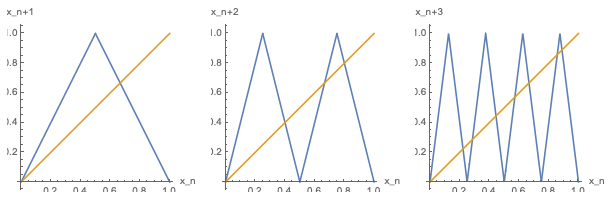
\includegraphics[width=0.9\textwidth]{img/C25-26p1a.png}

\end{questions}

\vspace{0.2cm}

\hrule
\vspace{0.2cm}

\noindent\textbf{Skill check C26 practice solution}
Two.

There are two period-1 points that will show up in the $x_{n+3}$ vs $x_n$ plot.  There is a period-2 orbit, but it won't show up in the $x_{n+3}$ vs $x_n$ plot.

There are eight fixed points in the $x_{n+3}$ vs $x_n$ plot.  Two of those are the period-1 points.  So six of those are period-3 points.  Six period-3 points corresponds to two period-3 orbits.


\vspace{0.2cm}

\hrule
\vspace{0.2cm}
\noindent\textbf{Questions}

\noindent \ \ 0.  Again today, share whatever you would like to, and write your names on the slide.

\begin{questions}

\question 
\begin{parts}
\item A period-2 orbit already exists at $r = 3.25$.  Based on the graphs below, between which two values of $r$ does a period-4 orbit develop?

$r = 3.25$

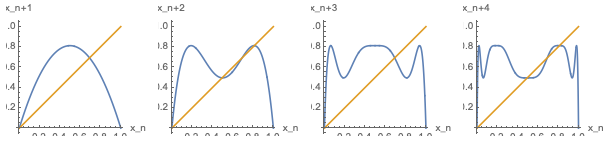
\includegraphics[width=0.9\textwidth]{img/C25-3-25-p1a.png}

$r = 3.35$

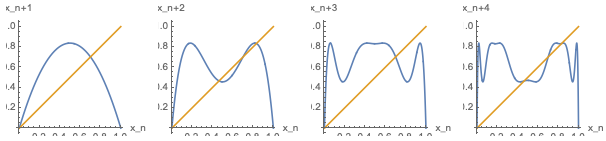
\includegraphics[width=0.9\textwidth]{img/C25-3-35-p1b.png}

$r = 3.45$

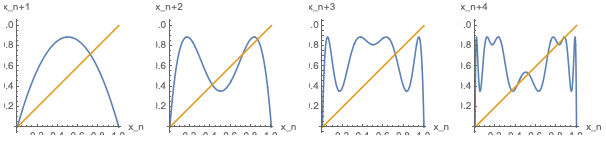
\includegraphics[width=0.9\textwidth]{img/C25-3-45-p1c.png}

$r = 3.55$

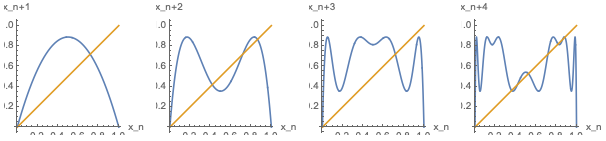
\includegraphics[width=0.9\textwidth]{img/C25-3-55-p1d.png}

$r = 3.65$

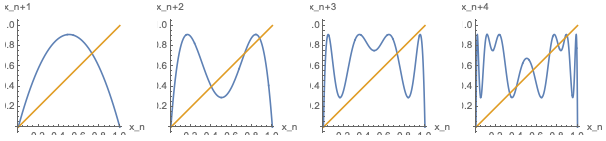
\includegraphics[width=0.9\textwidth]{img/C25-3-65-p1e.png}

\item What happens to the shapes of the plots above as $r$ increases?

\item On the left is a bifurcation diagram for the logistic map, $f(x) = rx(1-x)$.  I wasn't able to go beyond $r = 3.5$ because Mathematica got stuck on the algebra.  On the right is an orbit diagram for $0\leq r \leq 3.56$.

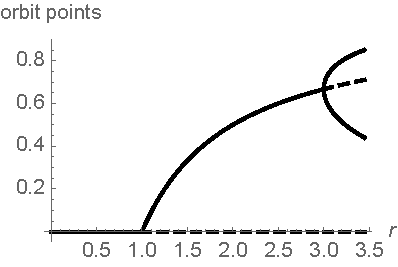
\includegraphics{img/191105-C26p4.pdf}
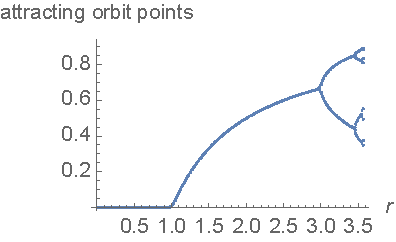
\includegraphics{img/191105-C26p5.pdf}

The \textbf{orbit diagram} is similar to a bifurcation diagram, but it does not show unstable fixed points or cycles, only stable ones.

Based on the orbit diagram, approximate the values of $r$ where a stable period-2 orbit and a stable period-4 orbit arise.

\end{parts}

\question (Exploring the orbit diagram for the logistic map) The logistic map is given by $f(x) = rx(1-x)$.  

\begin{parts}
\part  Below I plot the orbit diagram for the logistic map on the left for $0\leq r \leq 3.57$.  On the right, I zoom in on the region in the blue rectangle ($2.98\leq r \leq 3.57$).  

I made this diagram by using a single initial condition at each value of $r$, so all the points you see are part of the same period-k orbit.

At $r = 3$, you're seeing a period doubling bifurcation and the appearance of a period-2 orbit.
\begin{enumerate}
\item Looking closely at the plot on the right, how many period-doubling bifurcations do you see?
\item Identify the highest period object that you can see easily in the plot on the right.  How many points are involved in the orbit?
\end{enumerate}

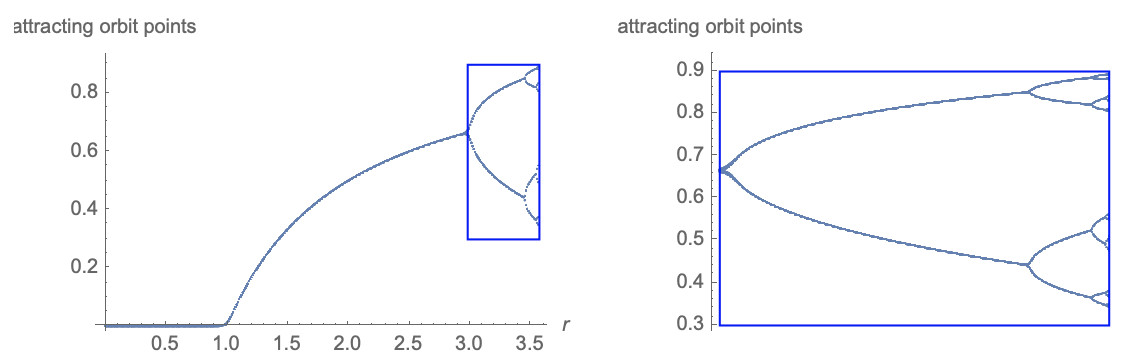
\includegraphics[width=0.9\textwidth]{img/191105-C26p6a.png}

\part  I zoom in again, taking a small corner of the blue box ($3.44\leq r \leq 3.57$), and marking it in red.  
 
 In red, I have cut off the upper part: if you see a period-2 orbit in the red zoomed-in area, it's actually a period-4 orbit.  What is the highest period orbit you can see now?


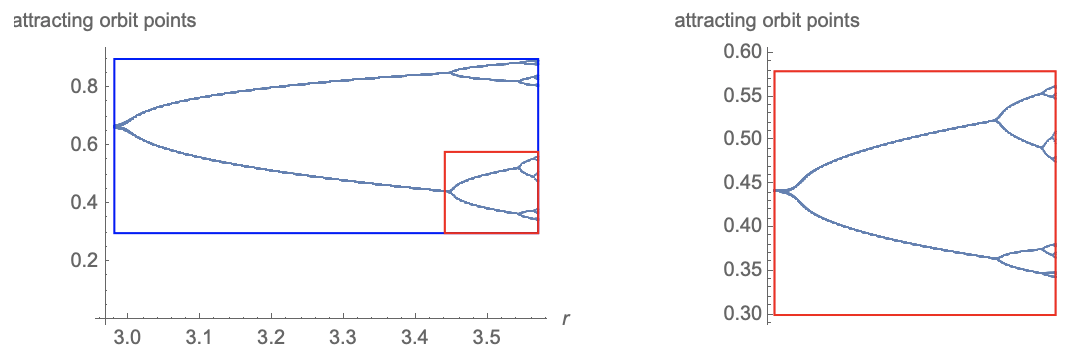
\includegraphics[width=0.9\textwidth]{img/191105-C26p6b.png}

\part  I zoom in again, taking a small corner of the red box ($3.54\leq r \leq 3.57$).  
 
 I have cut off the upper part: if you see a period-2 orbit in the magenta zoomed-in area, it's a period-4 in the red region, so actually a period-8 orbit.  What is the highest period orbit you can see now?

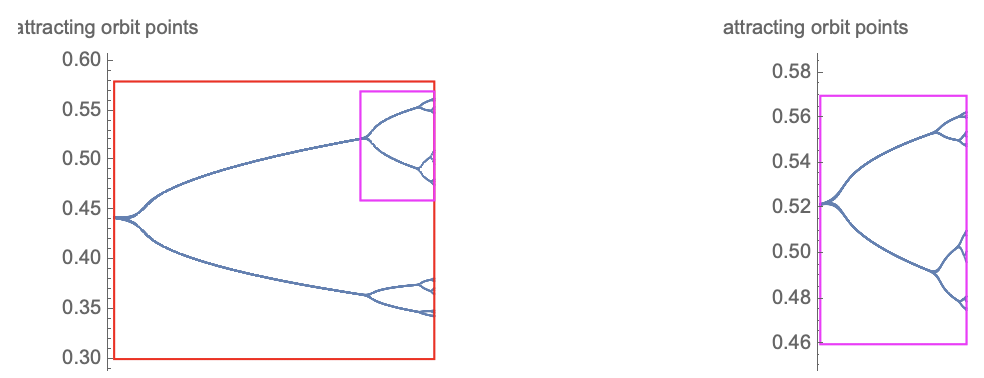
\includegraphics[width=0.9\textwidth]{img/191105-C26p6c.png}

\part  I zoom in one last time, taking a small corner of the magenta box ($3.54\leq r \leq 3.57$).  
 
 I have cut off the upper part: if you see a period-2 orbit in the orange zoomed-in area, it's a period-4 in the magenta region, so a period-8 orbit in the red, and actually a period-16 orbit.  What is the highest period orbit you can see now?

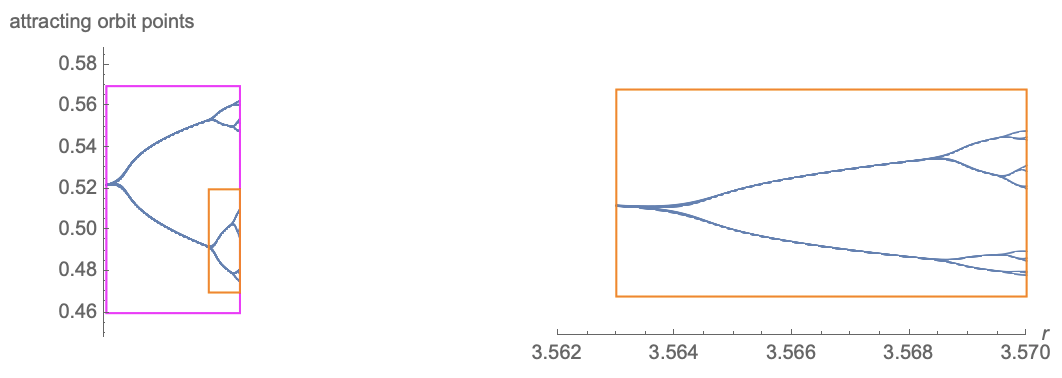
\includegraphics[width=0.9\textwidth]{img/191105-C26p6d.png}
\end{parts}

This sequence of bifurcation is called a \textbf{period-doubling cascade}.

\question A more extensive orbit diagram for the logistic map is shown below.

The ``fuzzy'' areas correspond to values of $r$ where there is a chaotic attractor.

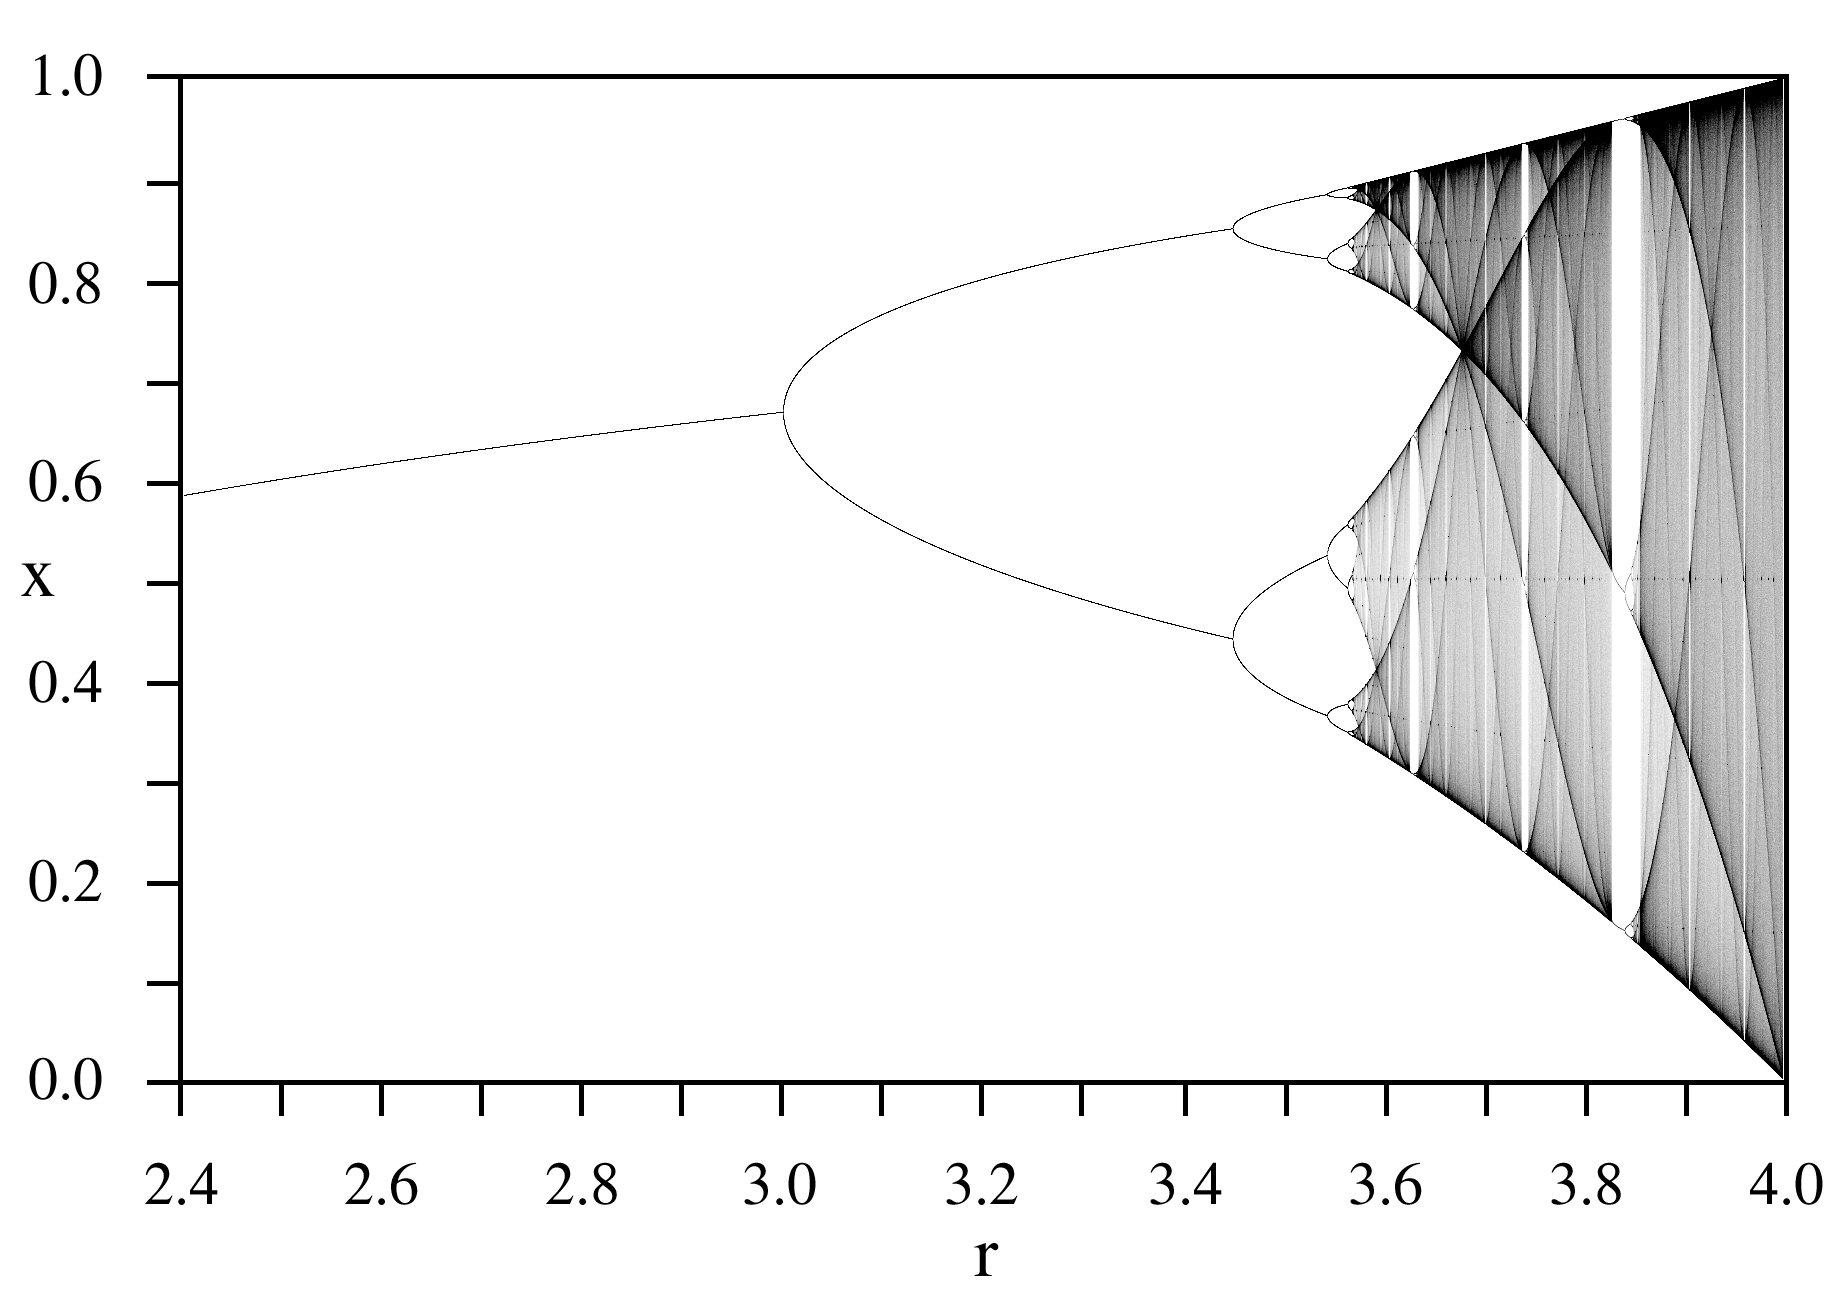
\includegraphics[width=6in]{img/logistic.png}

\begin{parts}
\item Take a look at the white areas that appear intermittently after $r=3.57$.  These are called \textbf{periodic windows}.  Can you find a white area that is a period-3 orbit?  What about a period-6?  How many periodic windows do you see?
\item(10.3.13) In the logistic orbit diagram above there are dark tracks of points running through the chaotic regions.  The logistic map is given by $x_{n+1} = rx_n(1-x_n)$.  The function $f(x; r) = rx(1-x)$ has its maximum at $x=\frac{1}{2}$.  Many values of $x$ map reasonably close to the maximum value of the map.  Why would that be?

\item This means that many values of $x$ map to close to $f(\frac{1}{2}; r) = \frac{r}{4}$.   One of these dark tracks is the curve $(r, f(\frac{1}{2},r))$.  What are the other curves?

\emph{Think about the map $g(x) = f(f(x))$}.
\item Set up an equation to find the value of $r$ at the corner where a bunch of the dark track intersect.

\emph{This corner involves $f^3$ and $f^4$.  Let $u = f^3(1/2; r)$ and $u = f^4(1/2; r)$.  Work with these to find an equation in terms of just $r$.}

\end{parts}

\end{questions}
\eject 


2a: I see a period-2, a period-4, a period-8 (and maybe a faint period-16).

2b: I see a period-4, a period-8, a period-16.

2c: I see a period-8, a period-16, a period-32.

2d: I see a period-16, a period-32, a period-64, and actually, a period-128.



2e: $2^k$ as $k\rightarrow\infty$, so a ton

3a: there's a period 3 at about 3.8 and a period 6 at about 3.62 or so.  There are lots of those periodic windows.

3b: There's a wide range of $x$-values that are going to about the same $f(x)$ near the maximum, because $f'(x) = 0$ at the maximum, so nearby $x$ values are going to almost the same $f$ value.

3c: Since $f(x;r)$ is often near $r/4$, $f^2(x;r)$ is often near $f(r/4;r)$, etc.  These curves are given by $f^m(\frac{1}{2}; r)$.
\begin{verbatim}
Clear[r, x]
f[x_, r_] = r x (1 - x);
Plot[{f[0.5, r], f[f[0.5, r], r],  f[f[f[0.5, r], r], r], 
  f[ f[f[f[0.5, r], r], r], r], 
  f[f[ f[f[f[0.5, r], r], r], r], r]}, {r, 2.95, 4}]
\end{verbatim}

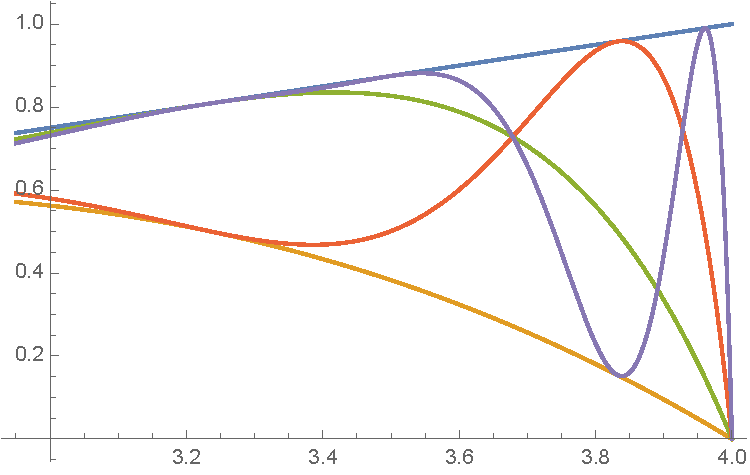
\includegraphics{img/17-04-12p1.pdf}

3d: At the intersection, $f^3(1/2;r) = f^4(1/2,r)$.  Let $u = f^3(1/2;r)$.  Then the intersection happens when $f(u,r) = u$.  This is a fixed point of the logistic map, so $u = 0$ or $u = 1-1/r$.  It must be that $u = 1-1/r$.  So $f^3(1/2;r) = 1-1/r$ is our equation.  Expanding:
\begin{verbatim}
Expand[f[f[f[1/2, r], r], r] - 1 + 1/r]
Solve[Expand[f[f[f[1/2., r], r], r] - 1 + 1/r] == 0, r]
\end{verbatim}
\[-1 + \frac{1}{r} + r^3/4-r^4/16-r^5/16+r^6/32-r^7/256=0.\]  This factors into $(r-2)^4(r+2)(r^3-2r^2-4r-8)=0$ so $r\approx 3.67857$.

\end{document}